\section{Additional Experiments Plan}
\label{section:Results:AdditionalExperimentalPlan}
% \todo[inline]{Her presser vi inn "Experiemnt Plan" og "Method" i samme seksjon. Blir det uryddig?}
% Tror ikke det er så uryddlig likevel. Virker som om Anders var fornøyd
After analyzing the initial results from our defined experiments
we formed some hypotheses, which led to some additional experiments.
These experiments are described in this section.

\subsection{Experiment 4: CNN-AE-LSTM on Noisy datasets}
\label{section:results:additional-experimental-plan:Experiment-4}
The CNN-AE-LSTM performed best on dataset 1, which we know
has the most noise. To confirm our hypothesis
that the CNN-AE-LSTM performs better than a LSTM
on the noisy dataset we add three new datasets,
one set consists of noisy time series,
the other consists of time series with low noise.
In fear that the noisiest dataset would be too noisy to give any meaningfule
predictions we added the third dataset, which has above-average noise, but not
as much as the noisiest data set.

% Here we briefly describe the methodology behind the experiment.

\subsubsection{Choosing the datasets}
To make the two datasets we looked at the standard deviation.
Firstly we scaled down outliers which could skew the standard deviation of
a series to be higher. For this we used the same technique
as described in \Cref{section:Data:Preprocessing:scale-down-outliers}.

Then, for each time series in the whole dataset we did these steps
\begin{enumerate}
  \item Scale down the values to have a mean of 0 using standardization.
  \item Take the difference of $t_n - t_{n-1}$
  \item if the standard deviation of the remaining series is above $max\_threshold$ \-\> Add to max list
  \item if the standard deviation of the remaining series is below the $min\_threshold$ \-\> Add to min list
\end{enumerate}

The noisiest dataset had standard deviation above $max\_threshold = 1.3$.
The dataset with the least noise had a standard deviation below $min\_threshold = 0.4$.
The above average noisy dataset had a standard deviation above $ok\_threshold = 0.8$
but below the maximum threshold of 1.3.
From the remaining list we randomly picked 7 time series.
Examples from each dataset is shown in \Cref{fig:time-series-variance-examples},
and the full list of categories are presented in
\Cref{table:dataset-high_variance_categories},
\Cref{table:dataset-low_variance_categories},
and \Cref{table:dataset-ok_variance_categories}.

\begin{figure}[h!]
  \centering
  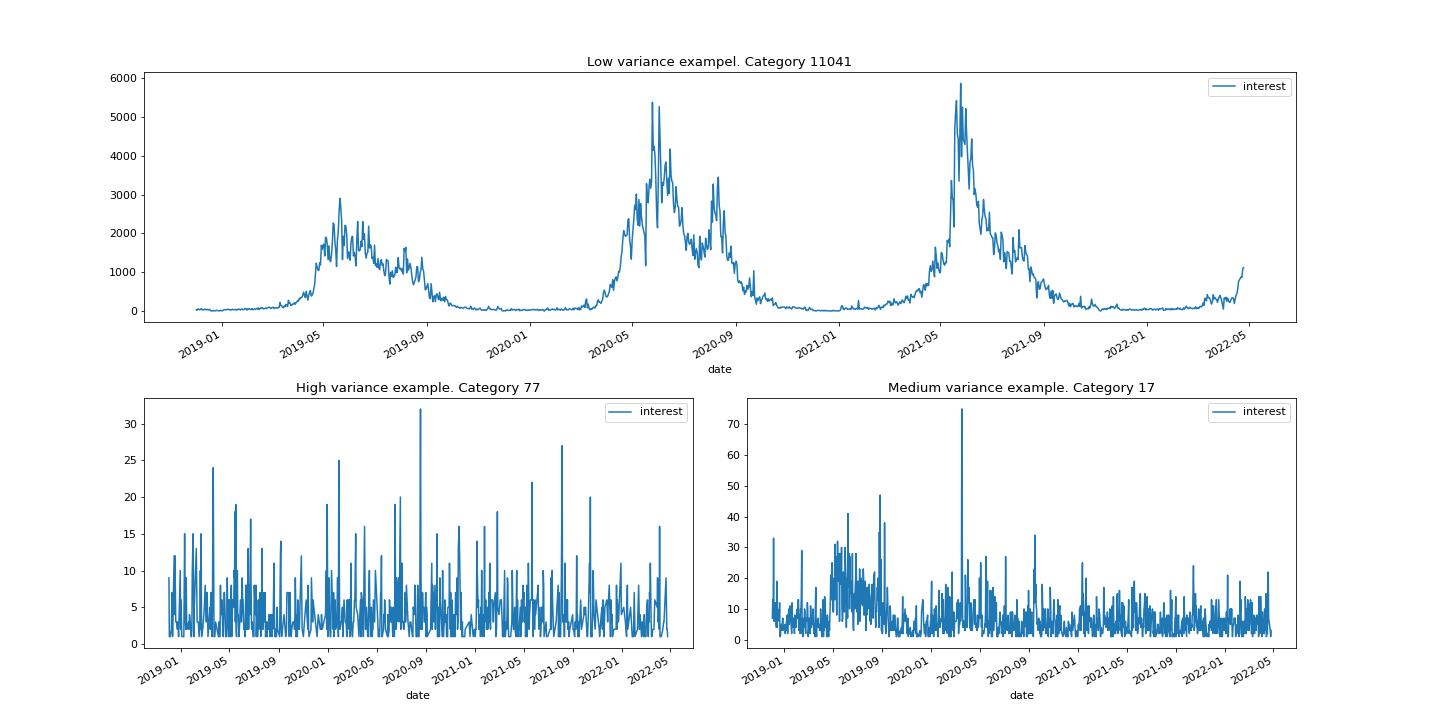
\includegraphics[width=\textwidth]{./figs/code_generated/time-series-variance-examples.png}
  \hfill
  \caption{Illustration of time series from the low variance dataset (top), high variance (bottom left), and the medium variance dataset (bottom right).}
  \label{fig:time-series-variance-examples}
\end{figure}

% Datasets
\import{./tables/code_generated/data_exploration}{dataset-high_variance_categories.tex}
\import{./tables/code_generated/data_exploration}{dataset-low_variance_categories.tex}
\import{./tables/code_generated/data_exploration}{dataset-ok_variance_categories.tex}

\subsubsection{Running the experiments}
The only two model structures we use are local univariate LSTM
and local univariate CNN-AE-LSTM.
We follow the same procedure as previously described in \Cref{section:Method},
except we do not tune the hyperparameters. Instead, we
use a hyperparameter-set from a previously tuned experiment and use those for all the models.
This is done because of time constraints.

\subsubsection{Experiment Plan}
\begin{description}
  \item[Outline]{
              Train and test a local univariate LSTM,
              and a local univariate CNN-AE-LSTM on a noisy dataset, a low noise dataset, and a medium noisy dataset,
              using MASE and sMAPE as metrics on a 7-day forecast.
              Compare the results against each other.
        }
\end{description}

\begin{description}
  \item[Expectations]{
              We expect the CNN-AE-LSTM to outperform the LSTM on the noisy datasets.
              We also expect the LSTM to have the best performance on the low noise datasets.
        }
\end{description}

\subsection{Experiment 5: Differencing on seasonal dataset}
\label{section:results:additional-experimental-plan:Experiment-5}
The literature on RNN's ability to model seasonality was conflicting [\Cref{section:Data:Preprocessing:trend-and-seasonality}].
Our initial results showed that the LSTM suffered on datasets with strong yearly seasonality.
We want to test if removing trends and seasonality can improve forecasts.

\subsubsection{Choosing Datasets}
We chose dataset 3 as the main dataset and dataset 1 as a control dataset.
Dataset 3 consists of series with strong seasonality, while dataset 1 has a relatively low seasonality.

\subsubsection{Removing Trend and Seasonality}
To remove the trend and seasonality from the time series
we use differencing transformation, which is a method of transforming a time series,
which removes its temporal dependence \cite[p. 215]{RobJHyndman2014}.
STL decomposition was tested as well, but it proved to be give worse results than with differencing.
Differencing is performed by subtracting the previous observation from the current
observation as shown in \Cref{eq:differencing} where $z$ is the
transformed differenced series, and $y$ is the real observations.
\begin{equation}
  \text{z}(t) = y(t_n) - \text{y}(t_{ n-1 })
  \label{eq:differencing}
\end{equation}

The transformation can be removed with \Cref{eq:differencing-inverted}.
\begin{equation}
  \hat{y}(t) = z(t_n) + y(t_{ n-1 })
  \label{eq:differencing-inverted}
\end{equation}

\subsubsection{Running the experiments}
We would follow the same experimental procedure as previously described in \Cref{section:Method},
except for section \Cref{section:Data:Preprocessing:trend-and-seasonality} which we replace with differencing described above.


\subsubsection{Experiment Plan}
\begin{description}
  \item[Outline]{
              Tune, train and test a local univariate LSTM with differencing
              on dataset 1 and 3,
              using MASE and sMAPE as metrics on a 7-day forecast.
              Compare the results against previously ran experiment without differencing.
        }
\end{description}

\begin{description}
  \item[Expectations]{
              We expect the LSTM with differencing to perform better on dataset 3.
              We do not know how differencing will affect the results on dataset 1.
        }
\end{description}


